\documentclass[11pt]{article}
\usepackage[utf8]{inputenc}
\usepackage{graphicx}
\usepackage{caption}
\usepackage{subcaption}
\usepackage{amsmath}
\usepackage{float}


\title{
	{Computer Vision 2 - Assignment 1\\
	 Iterative Closest Point - ICP}
}
\author{
Selene Baez Santamaria (10985417) - Ildefonso Ferreira ()}
\date{\today}

\begin{document}

\maketitle

\section{ICP}
In this assignment we create a function called \textit{own\_ICP} which implements the Iterative Closest Point algorithm. This function takes as arguments a base point cloud and a target point cloud, and a parameter $k$ for the number of points to be sampled. It outputs the base point cloud, the transformed point cloud, and the rotation and transformation matrices.

\subsection{Implementation}
Our implementation follows the basic steps outlined by \texttt{Cai et al}. The steps are further explained in the following list:

\begin{enumerate}
	\item \textbf{Find closest points:} In this phase we find the corresponding points in the clouds. To do so we use the function provided by the assignment package \textit{dist2} to find the distance among two sets of points. For each point in the base cloud we match it with the point in the target cloud that returns the lowest distance. 
	
	Our first approach was to use brute force and compare all points in one cloud to the points in the second cloud. However, this lead to problems regarding memory capacity. Thus, we chose to sample the points to be matched to work within such limitations.
	
	A second approach led us to sample the first \textit{k} elements in each cloud and compare them. This leas to incomplete clouds which were not representative of the whole.
	
	Finally, we decided to go with uniform random sampling to get $k$ samples from each cloud, and match them together. This by itself brings new problems which shall be discussed in Section \ref{reflection}
	
	\item \textbf{Center point clouds:} Secondly, we find the geometric centers of each cloud and subtract the centroid from each point. 
	
	For the base point cloud we only calculate and shift the cloud once, in the first iteration of the algorithm. Since the base cloud does not change over the iterations, there is no need to recalculate this process.
	
	On the other hand, since the matched points from the target cloud do change, we calculate the centroid for this matched cloud on every iteration and subtract it from every point.
	
	\item \textbf{Matrix Decomposition:} Next, we apply Singular Value Decomposition using Matlab's built in function \textit{svd}. The matrix to be decomposed is $A$, dimensions $3 x 3$, which is built as the dot product of the centered clouds: 
	
	\begin{center}
		$A = cen_pcd_b^T * cen_pcd_match$
	\end{center}
	
	The resulting matrices are the standard $U, S, V$ matrices.	
	
	\item \textbf{Find transformation matrices:} We proceed to calculate the Rotation and Translation matrices. 
	
	Since at every iteration we perform an update on the transformation of the target cloud, all of these updates must be combined to create the final matrices. For the rotation matrix this means each intermediate matrix should be multiplied with the accumulated matrix. For the translation matrix this means each intermediate matrix must be added to the accumulated matrix.
	
	\item \textbf{Transform matrix and evaluate:} Finally we calculate the average distances between the base and the transformed clouds. 
	
	We implemented two smart stopping conditions: the first stops if the distance is already within a certain threshold. The selected threshold is $ threshold = 0.00005 $. The second condition limits the number of iterations to $50$, since literature shows that this is often where the rate of significant improvement slows down.
\end{enumerate}

We tested our implementation with the given \textit{source.mat} and \textit{target.mat} files. In Figure \ref{fig:test} we present a visualization of the results obtained with these point clouds while Figure \ref{fig:test_performance} shows the performance on the algorithm per iteration.

\begin{figure}[H]
	\centering
	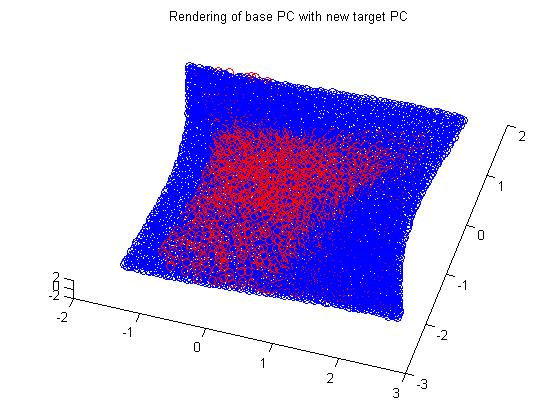
\includegraphics[width=.6\textwidth]{img/test_clouds.jpg}
	\caption{Alignment of source and target point clouds provided. Blue points correspond to source cloud and green points correspond to target cloud}
	\label{fig:test}
\end{figure}

\begin{figure}[H]
	\centering
	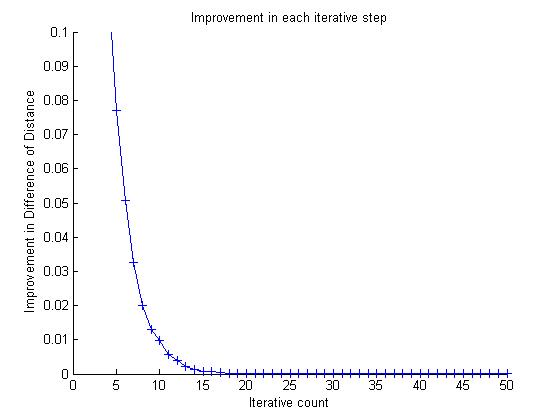
\includegraphics[width=.6\textwidth]{img/test_performance.jpg}
	\caption{Average distance between matched points per iteration for source and target test datasets.}
	\label{fig:test_performance}
\end{figure}


\section{Merging scenes}
We use our function on the dataset provided. Each point cloud corresponds to the image of a person from different angles. 


\subsection{Estimating camera poses using consecutive frames}



\subsection{Estimating camera poses using iterative merging}



\section{Discussion}
\label{reflection}
Given the previous results we can reflect on our implementation and on the ICP algorithm in general.

\subsection{Drawbacks of ICP}
Sampling size is important. Given the memory complexity of the brute force comparison, we have to work within a certain limit of comparisons.

The performance heavily depends on the initial orientation of the point clouds. 

Normalization does not change the performance.
 
 
\subsection{Improvements}
With regards to our implementation, we recognize that the sampling process could be improved. A smarter approach is to get the most significant points from the clouds and compare them, instead of choosing random points. 



\end{document}

